\begin{homeworkProblem}

Adopt the Acceptance-Rejection method to estimate the value of $\pi$, then evaluate the performance of Monte Carlo algorithms with finite number of samples.

\textcolor{blue}{Solution} \\

We can estimate $\pi$ via Monte Carlo method. Sample $X, Y\stackrel{i.i.d.}{\sim}\Unif(0,1)$. If $(x,y)$ is in the unit circle in the first quadrant, then $x^2+y^2\leq 1$, we count the number of these points as $N_{\text{in}}$. Then the estimatied $\hat{\pi}=4\cdot\dfrac{N_{\text{in}}}{N}$, where $N$ is the total number of sample points.

The number of sample points $N$ are set to be $10, 10^2, 10^3, 10^4, 10^5, 10^6$ respectively. The results are shown in the following figure, the estimated $\hat{\pi}$, estimation error $|\hat{\pi}-\pi|$. We could discover that more sample points could lead to a more accurate estimation of $\pi$.

\begin{figure}[h]
    \centering
    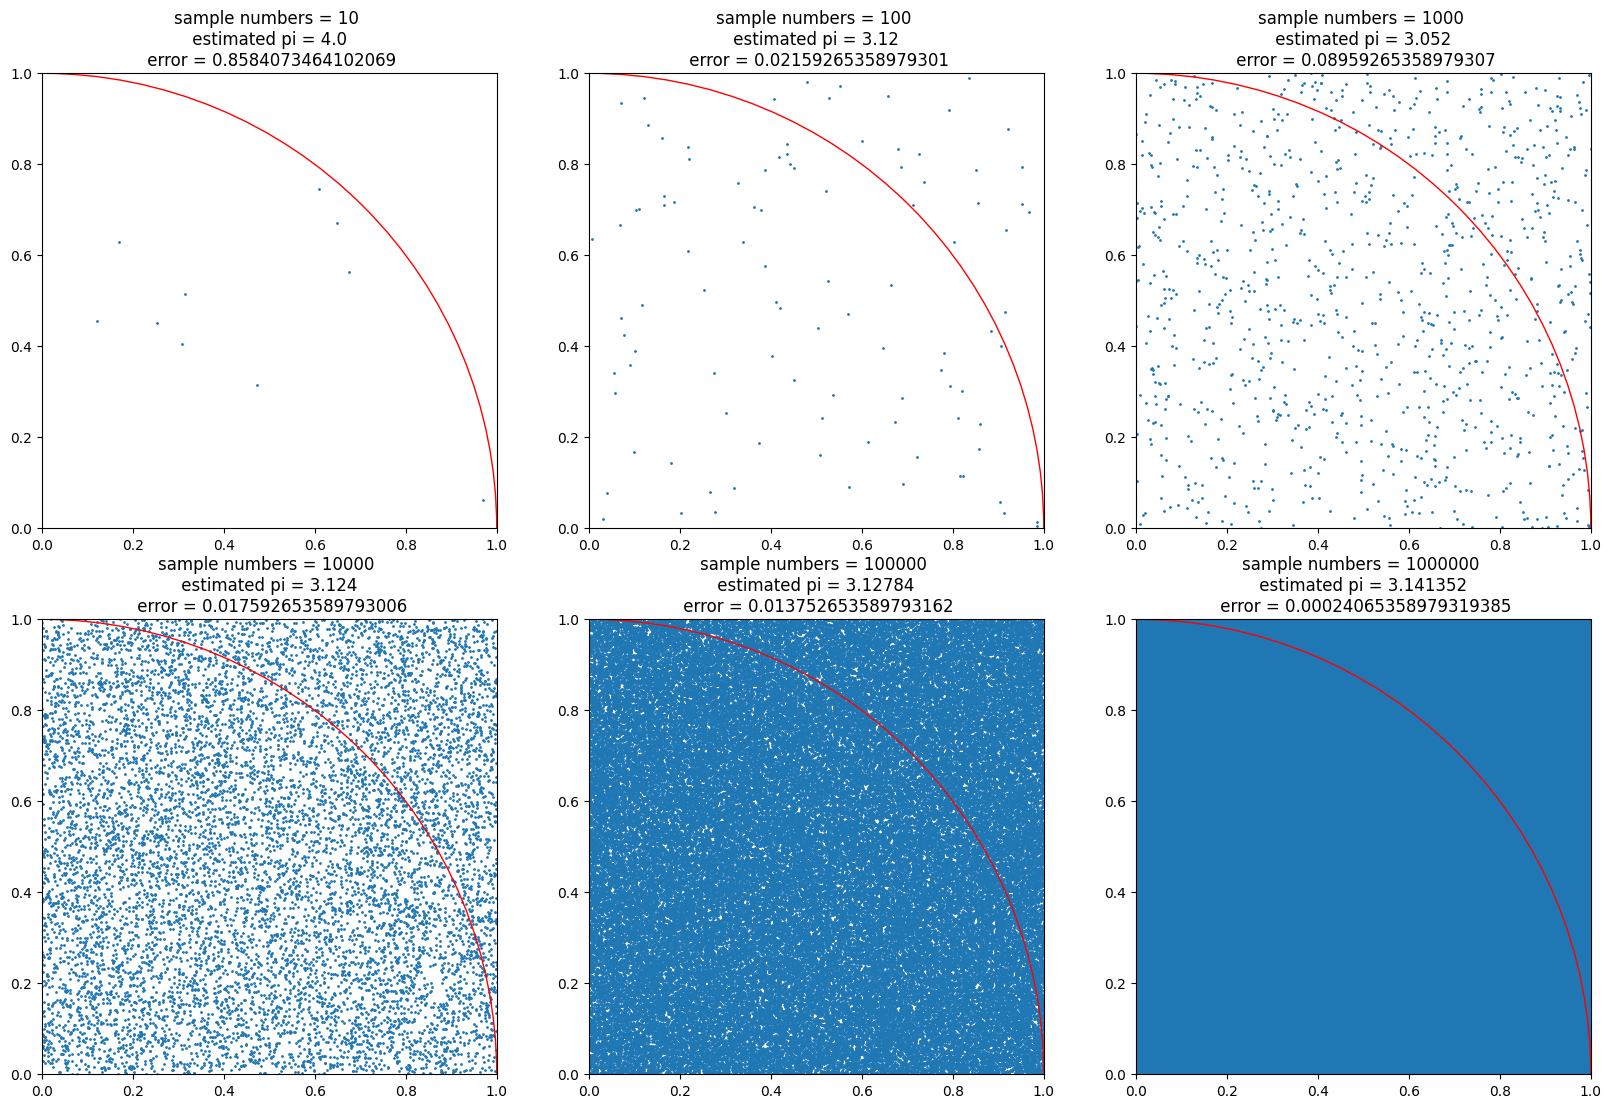
\includegraphics[width=\textwidth]{./figure/p4/simulated_result.png}
    \caption{The estimation of $\pi$ via Monte Carlo method}
\end{figure}

Let $Z_i=\I\{\text{The i-th sample is in the circle of the first quadrant}\}$. Then the estimated $\pi$ is
$$\hat{\pi}=4\cdot\dfrac{1}{n}\sum_{i=1}^n Z_i$$
The error probability can be calculated as
$$P\left(|\pi-\hat{\pi}|\geq \epsilon \right) = P\left(\left|\dfrac{4}{n}\sum_{i=1}^n Z_i-\pi\right|\geq\epsilon\right)=P\left(\left|\dfrac{1}{n}\sum_{i=1}^n Z_i-\dfrac{\pi}{4}\right|\geq\dfrac{\epsilon}{4}\right)$$
According to the Hoeffding's inequality, we have
$$P\left(\left|\sum_{i=1}^n Z_i-\dfrac{n\pi}{4}\right|\geq\dfrac{n\epsilon}{4}\right)\leq 2\exp\left(-\dfrac{2n\left(\frac{\epsilon}{4}\right)^2}{(1-0)^2}\right)=2e^{-\frac{1}{8}n\epsilon^2}=\delta$$
Where $1-\delta$ is the confidence level. So we can get that $\epsilon = \sqrt{\dfrac{8\ln\dfrac{2}{\delta}}{n}}$. Which means that
$$P\left(\pi\in\left(\hat{\pi}-\sqrt{\dfrac{8\ln\dfrac{2}{\delta}}{n}}, \hat{\pi}+\sqrt{\dfrac{8\ln\dfrac{2}{\delta}}{n}}\right)\right)\geq 1-\delta$$

Here we set $\delta=0.05$, which means that we have a $95\%$ confidence level that the estimated $\pi$ is in the interval. The upper bound and lower bound of the interval are shown in the following figure. And we can see that the estimated $\hat{\pi}$ has mostly been in the interval.

\begin{figure}[h]
    \centering
    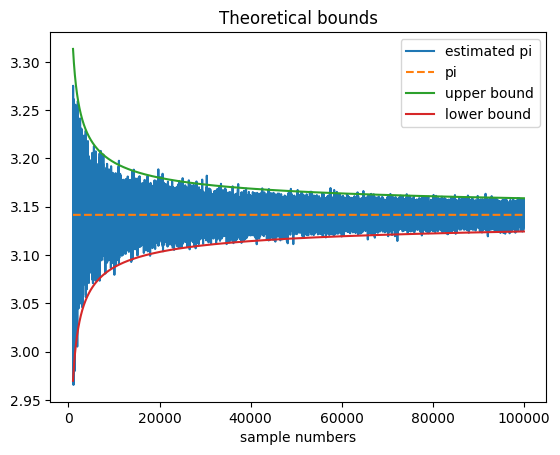
\includegraphics[width=0.8\textwidth]{./figure/p4/analysis.png}
    \caption{Analysis the performance of the estimated $\hat{\pi}$}
\end{figure}

\end{homeworkProblem}

\newpage